% vim: set textwidth=78 autoindent:

\subsection{OpenStreetMap Plugin}

% when the revision of a section has been finalized, 
% comment out the following line:
% \updatedisclaimer

In recent years the OpenStreetMap project has gained popularity because in 
many countries no free geo data such as digital roadmaps are available. 
Target of the OSM project is to create a free editable map of the world 
from GPS data, aerial photography or simply from local knowledge. To 
support this idea QGIS provides a plugin that enables its users to work
with OSM data.

The plugin provides all basic functionalities for OSM data manipulation, 
such as data loading, importing, saving, downloading, editing and 
uploading data back to the OpenStreetMap server. While implementing OSM 
plugin an inspiration was taken from existing OSM data editors. The 
purpose was to combine their functionalities to get the best
possible result.

The following subsection gives a brief introduction to principles of the OSM 
project. If you are not interested in information on OSM just skip the next 
section. Parts of the following paragraphs are copied from the 
OpenStreetMap web site.

\minisec{The OpenStreetMap project}

OpenStreetMap is a project to create a free editable map of the world. The
maps are created using data from portable GPS devices, aerial photography,
other free sources or simply from local knowledge. The project was started
because most maps have legal or technical restrictions on their use, holding
back people from using them in creative, productive, or unexpected ways. Both
rendered images and the vector dataset of OSM are available for download
under a Creative Commons Attribution ShareAlike 2.0 licence.

\begin{figure}[ht]
   \begin{center}
   \caption{OpenStreetMap data in the web \nixcaption}\label{fig:osmweb}\smallskip
   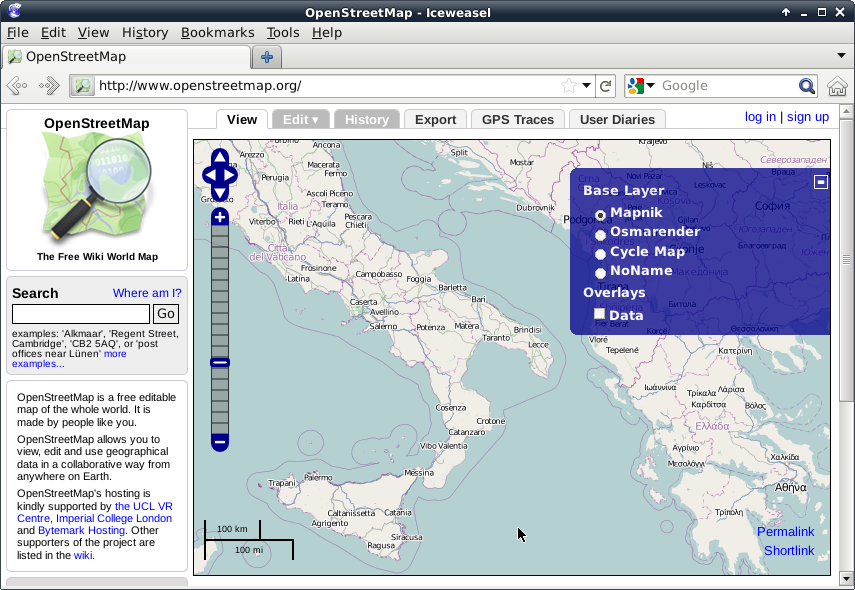
\includegraphics[clip=true, width=\textwidth]{osmweb}
\end{center}
\end{figure}

OpenStreetMap was inspired by sites such as Wikipedia - the map display 
(see Figure \ref{fig:osmweb}) features a prominent \tab{Edit} tab and a 
full revision history is maintained. Registered users can upload GPS track 
logs and edit the vector data using the given editing tools.

OSM data primitive is an object class that can be stored via the API in the
server. Three supported types of data are: \textbf{Node}, \textbf{Way} and 
\textbf{Relation}. 

\begin{itemize}
\item \textbf{A node} is a latitude/longitude pair of coordinates. It is 
used as building a block for other features and a feature itself (Points Of 
Interest) if they are tagged as required. 
\item \textbf{A way} is a list of at least two nodes that describe a linear
feature such as a street, or similar. Nodes can be members of multiple ways.
\item \textbf{A relation} is a group of zero or more primitives with 
associated roles. It is used to specify relationships between objects, 
and may also model an abstract object. 
\end{itemize}

Several different logical features in a common map ('Point Of Interest',
'Street', 'Tram Line', 'Bus Stop' etc.) are defined by these primitives. 
Map features are well-known in the OSM community and are stored as tags, 
based of a key and a value. OSM is usually distibuted in XML format. XML 
payload is used for the communication with the OSM server as well.

For more information visit the project website at:
\url{http://www.openstreetmap.org}.

\minisec{QGIS - OSM Connection}\label{qgis-osm-connection}

The first part of this subsection describes the way how OSM data primitives 
are displayed in QGIS vector layers.

As written above, OSM data consist of Nodes, Ways and Relations. In QGIS they 
are displayed in three diffrent layer types: Point layer, Line layer and 
Polygon layer. It's not possible to remove any of these layers and work with 
the other ones.

\begin{itemize}
\item \textbf{Point layer} displays all features of type Node that stands 
alone. That means that only Nodes that are not included in any Way belongs 
to the Point layer.
\item \textbf{Line layer} displays those OSM features of type Way that are 
not closed. That means that none of these Ways starts and ends with the 
same Node.
\item \textbf{Polygon layer} displayes all Ways that are not included in 
Line layer.
\end{itemize}

OpenStreetMap has one more data primitive except for the three mentioned
above - Relation. In our design there is purposely no vector layer to display
Relations. Relation defines relation between any number of data primitives.
After Point, Line or Polygon is identified on map, plugin shows a list of all
relations the identified feature is part of.

Challenging was designing the interconnection between OSM data and the 
standard QGIS editing tools. These tools are made to edit a single vector 
layer at a time, no matter of what feature types it displays. It means 
that if OSM data are loaded to QGIS through the plugin, you could 
(theoretically) edit Point layer, Line layer or Polygon layer with these 
standard tools separately.

The problem is that Line layer consists of two different types of OSM
features - Ways and Nodes. Why? Because in OSM format a \texttt{Way} is 
composed of Nodes. If you start editing a Line layer and change the 
shape of some line, your action must affect not only the OSM Way but 
also the OSM Nodes that are part of it. \\
QGIS standard editing tools cannot tell the OSM Provider which members
of which line has changed and how. It can tell only what's the new geometry
of which line, and that's not enough to propagate changes to OSM database
correctly. The Line layer does also not know identifiers of line members.
The same problem occurs when you try to edit the Polygon layer.

For this reason, the OSM plugin need its own simple tools for editing 
OSM data. While they are used, the OSM layers can be changed correctly. 
The Plugin editing set consists of tools for Point, Line, Polygon and 
Relation creation, deletion and moving.

\textbf{Note:} To create a connection between the OSM plugin and standard 
editing tools, changes in QuantumGIS core code would be necessary.

\subsubsection{Installation}

The OpenStreetMap plugin is a core plugin inside the QGIS environment. If 
you have python support enabled, the 'OpenStreetMap' plugin can be selected 
in the Plugin Manager as described in section \ref{sec:load_core_plugin}). 

\subsubsection{Basic user interface}

The first time the OSM plugin is started (and after the first data are 
loaded), several new OSM plugin icons appear in the QGIS toolbar menu 
together with new graphical components as shown in Figure 
\ref{fig:osmwidget}:

\begin{figure}[ht]
   \begin{center}
   \caption{OSM plugin user interface \nixcaption}\label{fig:osmwidget}\smallskip
   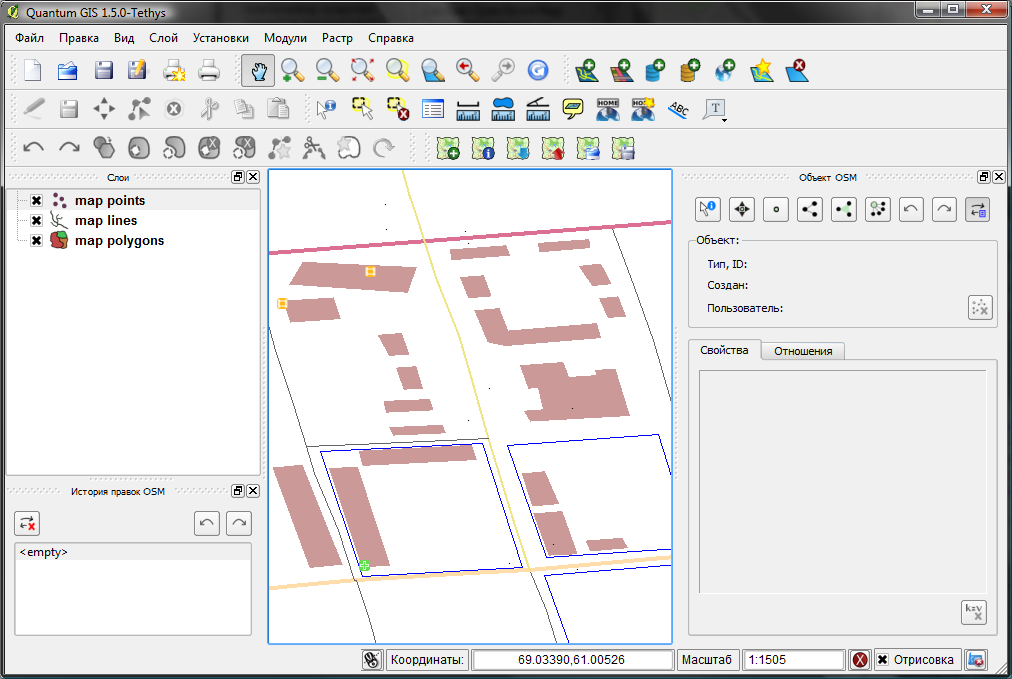
\includegraphics[clip=true, width=\textwidth]{osm_widgets}
\end{center}
\end{figure}

\minisec{OSM Features widget}

This widget helps to identify OSM features. It
shows basic information on features type and identifier as well as info on
who and when changed feature lately. OSM Feature widget holds all editing
tools also (in the top part of it). More information on those tools can be
found in section focused on editing. Widget is initially disabled. It
activates itself after successfull loading of some OSM data.

\minisec{OSM Undo/Redo widget}

This widget is used to undo and redo edit actions. It consists not only 
of clasical Undo button and Redo button, it shows a list with brief 
description of edit actions that were done. The OSM Undo/Redo widget
is initially closed. You can show it using special button on OSM Feature
widget.

\minisec{Toolbar menu icons}

\begin{description}
\item \toolbtntwo{osm_load}{Load OSM from file}: is used to load data from a 
special OpenStreetMap XML file.
\item \toolbtntwo{osm_featureManager}{Show/Hide OSM Feature Manager} is 
used to show or hide the OSM Feature widget. The OSM Feature widget is a 
panel that helps with OSM feature identification and with OSM data editing.
\item \toolbtntwo{osm_download}{Download OSM data} is used to download data 
from the OpenStreetMap server.
\item \toolbtntwo{osm_upload}{Upload OSM data} is used to upload changes 
(on current data). 
\item \toolbtntwo{osm_import}{Import data from a layer} is used to import 
data from a vector layer. At least one vector layer must be loaded and 
current OSM data must be selected.
\item \toolbtntwo{osm_save}{Save OSM to file} is used to save OSM data 
back to an XML file.
\end{description}

More detailed information on all the widgets, buttons and dialogs can be
found in appropriate sections of this Guide according to their functionality
(editing, identification, etc.).

\subsubsection{Loading OSM data}

The first action that should be done after starting OSM Plugin is opening
data from OSM file, import them from the shapefile or downloading data from
OpenStreetMap server. Here we are focusing on the first mentioned action.
To load data from file use the \toolbtntwo{osm_load}{Load OSM from file} 
icon. If there is no such button, maybe someone disabled OpenStreetMap 
toolbar in your QGIS instalation. You can enable it again selecting
\mainmenuopt{Settings} > \mainmenuopt{Toolbars} > \dropmenuopt{OpenStreetMap}.

\begin{figure}[ht]
   \begin{center}
   \caption{Load OSM data dialog \nixcaption}\label{fig:osmload}\smallskip
   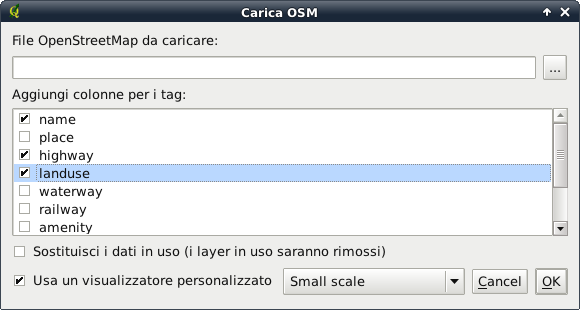
\includegraphics[clip=true, width=12cm]{osmloaddialog}
\end{center}
\end{figure}

Purpose of its elements is explained below.

\begin{description}
\item \textbf{OpenStreetMap file to load}: Click on the button to select 
the .osm file you want to load data from.
\item \textbf{Add columns for tags}: This option determines 
inter connection between OSM and QGIS data. Each feature of OSM data has 
some tags (pairs of key and value), that define the feature properties. 
Each feature of a QGIS vector layer also has its attributes (key and value). 
With this option you can define which properties of OSM objects should 
be visible when displaying detailed info about QGIS features.
\item \textbf{Replace current data}: Checking this option means that 
new data should replace current data user is working with. Layers of 
current data will be removed and new ones will be loaded. When loading 
first OSM data, this option is not active, because there is nothing 
to replace.
\item \textbf{Use custom renderer}: This option determines how rich will 
be the map in detail. The are three pre-defined OSM styles for map 
displaying. Use 'Small scale' if you want to view OSM data at low level, 
to see all details and to edit something. If not you can use 
'Medium scale' or 'Large scale'. At present days QGIS doesn't support 
changing renderer style dynamically.
\end{description}

Click \button{Ok} to load your data. If this is the first time OSM 
file is loaded, plugin must first parse it into database.
This may take few seconds or minutes - it depends on amount of loaded data.

\subsubsection{Viewing OSM data}

After OSM data were loaded you can identify map features using the
appropriate tool. Use the \toolbtntwo{osm_identify}{Identify feature} 
button on the top-left of OSM Feature widget. Using this tool you can 
easily explore map objects. When the mouse cursor is over an object, 
you can see all information on it directly in the OSM Feature widget. 
There is also a dynamic rubberband displayed on the map so that the user 
is able to determine which feature is currently identified.

The Properties table of the widget contains of all feature tags. Clicking on 
the \tab{Relation tab} shows you list of all relations connected with
identified feature.

If you want to hold a feature for a while to be able to read its properties 
and relations, move the mouse cursor at the same time, try left-clicking 
while you are over it. Identification process will stop until next 
left-clicking.

Sometimes there are more than one feature at the point where left-clicking
was performed. This happens especially when clicking on cross-roads or if 
you didn't zoom enough into the map. In this situation only one of such 
features is identified (and marked with the rubberband) but the plugin 
remembers all of them. Then (still in the pause mode) you can change 
identified features cyclical with right-clicking.

\subsubsection{Editing basic OSM data}

In the title of this section 'basic data' means non-relation OSM features -
nodes and ways. If you prefer reading information on relations editing just
skip this section and read the next one.
 
Basic data editing is key part of OSM Plugin. You can change property,
position or shape of any existing basic feature, you can remove features or
add some new ones. All such changes on nodes and ways are remembered - both
for comfortable usage of Undo/Redo operations and for easy upload of  changes
to OpenStreetMap server.

\minisec{Changing feature tags}

Changing property/tag of OSM feature can be done directly in table of feature
tags. Tags table of basic feature can be found on OSM Feature widget. Don't
forget to identify feature first.

\begin{figure}[ht]
   \begin{center}
   \caption{Changing an OSM feature tag \nixcaption}\label{fig:osmchfeattag}\smallskip
   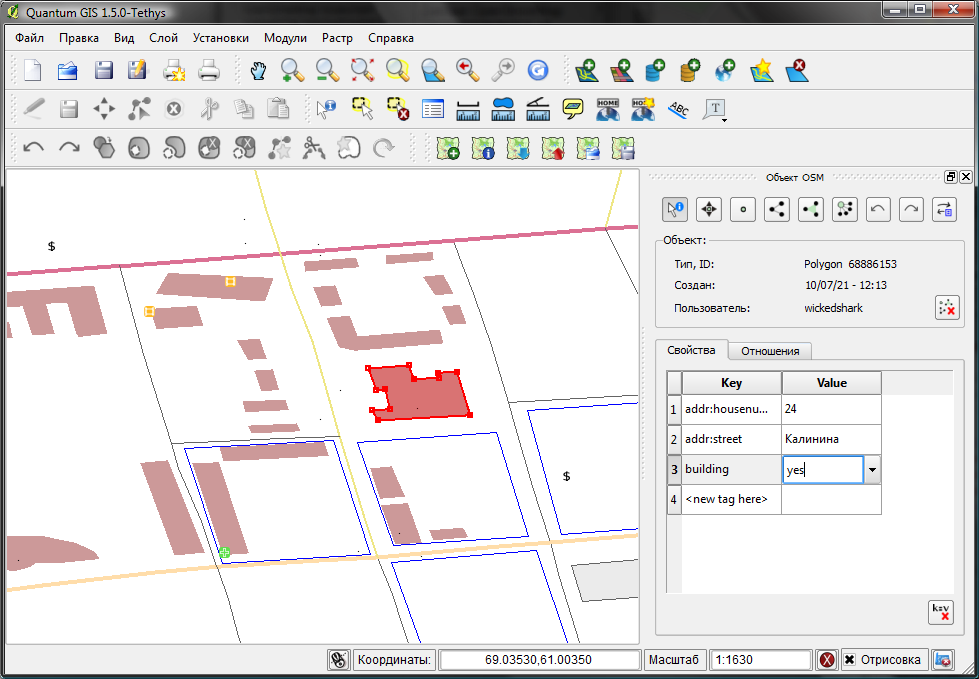
\includegraphics[clip=true, width=12cm]{osm_changefeaturetag}
\end{center}
\end{figure}

If you want to change tag value, just double-click in the appropriate row of
column Value and type or select new value. If you want to remove tag click in
its row, then use button on the right under the table - "Remove selected
tags"

To add new tag just type its key and value into the last row of the table -
where '<next tag value>' is written. Notice that you cannot change key of
existing tag pair. For comfortable usage there are some combo boxes of all
existing tag keys and their typical values.

\minisec{Point creation}

For point creation there is a \toolbtntwo{osm_createPoint}{Create point} 
button on OSM Feature widget. To create some points just click on the 
button and start clicking on the map. If your cursor is over some map 
feature, the feature is marked/identified immediately. If you click on 
the map when line/polygon is marked, new point is created directly on 
such line/polygon - as its new member. If your cursor is over an existing 
point, new point cannot be created. In such case OSM plugin will tell you:

\begin{figure}[ht]
   \begin{center}
   \caption{OSM point creation message \nixcaption}\label{fig:osmpoicreat}\smallskip
   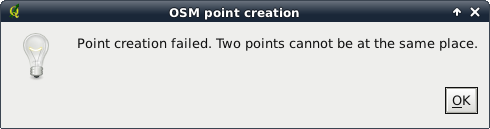
\includegraphics[clip=true, width=8cm]{osm_pointcreation}
\end{center}
\end{figure}

The mechanism of helping user to hit the line or polygon is called snapping
and is enabled by default. If you want to create point very close to some
line (but not on it) you must disable snapping by holding Ctrl key first.

\minisec{Line creation}

For line creation there is \toolbtntwo{osm_createLine}{Create line} button 
on OSM Feature widget. To create a line just click the button and start 
left-clicking on the map. Each your left-click is remembered as member 
vertex of new line. Line creation ends when first right-click is performed. 
New line will immediately appear on the map.

A Line with less than two members cannot be created. In such case the 
operation is ignored.

Snapping is performed to all map vertexes - points from Point vector layer
and all Line and Polygon members. Snapping can be disabled by holding 
\keystroke{Ctrl} key.

\minisec{Polygon creation}

For polygon creation there is \toolbtntwo{osm_createPolygon}{Create polygon} 
button on OSM Feature widget. To create a polygon just click the button 
and start left-clicking on the map. Each your left-click is remembered as 
member vertex of new polygon. Polygon creation ends when first right-click 
is performed. New polygon will immediately appear on the map.
Polygon with less than three members cannot be created. In such case
operation is ignored. Snapping is performed to all map vertexes - points 
(from Point vector layer) and all Line and Polygon members. Snapping can be 
disabled by holding \keystroke{Ctrl} key.

\minisec{Map feature moving}

If you want to move a feature (no matter what's its type) please use the
\toolbtntwo{osm_move}{Move feature} button from OSM Feature widget menu. 
Then you can browse the map (features are identified dynamically when you 
go over them) and click on the feature you want to move. If wrong feature is
selected after your click, don't move from the place. Repeat right-clicking
till the right feature is identified. When selection is done and you move
cursor you are no more able to change your decision what to move.
To confirm moving click with left mouse button. To cancel moving click 
with another one.

If you are moving a feature that is connected to other features, these
connections won't be damaged. Other features will just adapt themselves to
new position of moved feature.

Snapping is supported in this operation.

When moving a standalone (not part of any line/polygon) point, snapping to
all map segments and vertexes is performed.

When moving a point that is member of some lines/polygons, snapping to all
map segments and vertexes is performed, except for vertexes of point parents.

When moving a line/polygon, snapping to all map vertexes is performed. Note
that OSM Plugin tries to snap only 3 closest-to-cursor vertexes of moved
line/polygon, otherwise operation would by very slow.
Snapping can be disabled by holding Ctrl key during the operation.

\minisec{Map feature removing}

If you want to remove feature, you must identify it first. To remove 
identified feature use \toolbtntwo{osm_removeFeat}{Remove this feature} button 
on the OSM Feature widget. When removing a line/polygon, the line/polygon 
itself is deleted, so are all its member points that doesn't belong to any 
other line/polygon. When removing a point that is member of some 
lines/polygons, point is deleted and geometries of parent lines/polygons 
are changed. New parent geometries has less vertexes than the old ones.

If parent was a polygon with three vertexes, its new geometry has only two
vertexes. And because there cannot exist polygon with only two vertexes,
feature type is automatically changed to Line.

If parent was a line with two vertexes, its new geometry has only one vertex.
And because there cannot exist line with only one vertex, feature type is
automatically changed to Point.

\subsubsection{Editing relations}\label{editing_osm_relation}

Thanks to existency of OSM relations we can join OSM features into groups and
give them common properties - in such way we can model any possible map
object: borders of a region (as group of ways and points), road of a bus,
etc. Each member of relation has its specific role.
There is a pretty good support for OSM Relations in our plugin.
Let's see how to examine, create, update or remove them.

\minisec{Examining relation}

If you want to see relation properties, first identify one of its members.
After that open tab "Relations" on OSM Feature widget. At the top of the tab
you can see a list of all relations the identified feature is part of. Please
choose the one you want to examine and look at information thereunder.
In the first table called "Relation tags" there are properties of selected
relation.
In table called "Relation members" you can see brief info on relation
members.
If you click on a member, plugin will make a rubberband on it in map.

\minisec{Relation creation}

There are 2 ways of creating a relation. 

\begin{itemize}
\item You can use the \toolbtntwo{osm_createRelation}{Create relation} 
button on OSM Feature widget.
\item You can create it from the Relation tab of OSM Feature widget by 
using the \toolbtntwo{osm_addRelation}{Add relation} button.   
\end{itemize}

In both cases dialog will appear. In second case feature that is currently
identified is automatically considered to be the first relation member, so
dialog is pre-filled a little. When creating relation please select its 
type first. You can select one of predefined relation types or write your 
own type. After that fill relation tags and choose its members.

If you have relation type already selected try using the 
\toolbtntwo{osm_generateTags}{Generate tags} button. It will 
generate typical tags to your relation type. Then you are expected to 
enter values to the keys. Choosing relation members can 
be done either simply by writting member identifiers, types and roles or 
by using the \toolbtntwo{osm_identify}{identify} tool and clicking on map.
Finally when type, tags and members are chosen dialog can be submitted - in
such case plugin creates new relation for you.

\minisec{Changing relation}

If you want to change an existing relation, identify it first (follow steps
written above in Examining relation). After that click on the 
\toolbtntwo{osm_editRelation}{Edit relation} button, you will find it 
on OSM Feature widget. A new dialog appears, nearly the same as for the 
Create relation action. The dialog is pre-filled with information on 
given relation. You can change relation tags, members or even its type. 
After submiting the dialog your changes will be commited.

\subsubsection{Downloading OSM data}  

To download data from OpenStreetMap server click on the 
\toolbtntwo{osm_download}{Download OSM data} button. If there is no 
such button, the OSM toolbar may be disabled in your QGIS instalation.
You can enable it again at \mainmenuopt{Settings} > 
\mainmenuopt{Toolbars} > \dropmenuopt{OpenStreetMap}. After clicking the 
button a dialog occurs:

\begin{figure}[ht]
   \begin{center}
   \caption{OSM download dialog \nixcaption}\label{fig:osmdownload}\smallskip
   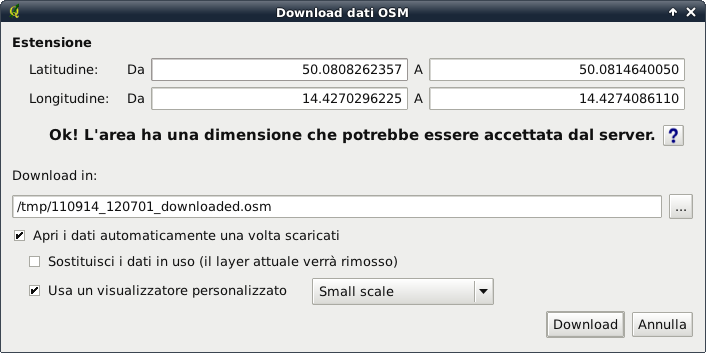
\includegraphics[clip=true, width=8cm]{osm_downloaddialog}
\end{center}
\end{figure}

\begin{description}
\item \textbf{Extent}: Specifies area to download data from - intervals 
of latitude and longitude degrees. Because there is some restriction of 
OpenStreetMap server on how much data can be downloaded, the intervals 
mustn't be too wide. More detailed info on extent specification can is 
shown after clicking the \toolbtntwo{osm_questionMark}{help} button on 
the right.
\item \textbf{Download to}: Here you are expected to write path to the file 
where data will be stored. If you can't remember structure of your disk, 
don't panic. The browse button will help you.
\item \textbf{Open data automatically after download}: Determines if 
download process should be followed by loading data process or not. If you 
prefer not to load data now, you can do it later by using 
the \toolbtntwo{osm_load}{Load OSM from file} button.
\item \textbf{Replace current data}: This option is active only if the 
'Open data automatically after download' is checked. Checking this option 
means that downloaded data should replace
current data we are working with now. Layers of current data will be removed
and new ones will be loaded. When starting QGIS and downloading first data
this option is initially inactive, because there is nothing to replace.
\item \textbf{Use custom renderer}: This option is active only if the 
'Open data automatically after download' checkbox is checked. It determines 
how rich will be the map in detail. The
are three predefined OSM styles for map displaying. Use 'Small scale' if you
want to view OSM data at low level, to see all details and to edit something.
If not you can use 'Medium scale' or 'Large scale'. At present days QGIS
doesn't support changing renderer style dynamically.
\end{description}

Click the \button{Download} button to start the download process.

A progress dialog will continuously inform you about how much of data is
already downloaded. When an error occure during download process dialog tell
you its details. When action finishes succesfully both the progress dialog
and download dialog will close themselves.

\subsubsection{Uploading OSM data}  

Note that upload is always done on current OSM data. Before opening OSM
Upload dialog, please be sure that you really have the right active layer ~
OSM data.

To upload current data to OSM server click on the 
\toolbtntwo{osm_upload}{Upload OSM data} button. If there is no such button, 
OSM toolbar in your QuantumGIS instalation is disabled. You can enable it 
again at \mainmenuopt{Settings} > \mainmenuopt{Toolbars} > 
\dropmenuopt{OpenStreetMap}. After clicking on upload button a new dialog 
will appear.

\begin{figure}[ht]
   \begin{center}
   \caption{OSM upload dialog \nixcaption}\label{fig:osmupload}\smallskip
   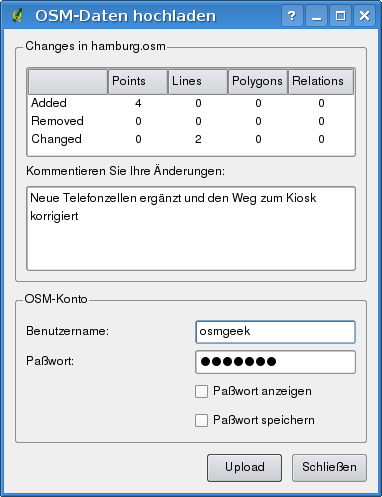
\includegraphics[clip=true, width=8cm]{osm_uploaddialog}
\end{center}
\end{figure}

At the top of dialog you can check if you are uploading correct data. There
is a short name of current database. In the table there is information on how
many changes will be uploaded. Statistics are displayed separately for each
feature type.
In 'Comment on your changes' box you can write brief information on meaning
of your upload operation. Just write in brief what data changes you've done
or let the box empty.
Fill 'OSM account' arrays so that server could authenticate you. If you don't
have account on OSM server, it's the best time to create one. Please visit
www.openstreetmap.org.
Use Upload to start an upload operation.

\subsubsection{Saving OSM data}  

To save data from current map extent to XML file click on 
\toolbtntwo{osm_save}{Save OSM to file} button. If there is no such button, 
OSM toolbar in your QuantumGIS instalation is disabled. You can enable it 
again at \mainmenuopt{Settings} > \mainmenuopt{Toolbars} >
\dropmenuopt{OpenStreetMap}. After click on the button a new dialog appears.

\begin{figure}[ht]
   \begin{center}
   \caption{OSM saving dialog \nixcaption}\label{fig:osmsave}\smallskip
   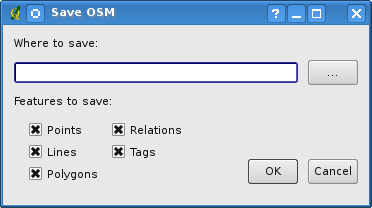
\includegraphics[clip=true, width=8cm]{osm_savedialog}
\end{center}
\end{figure}

Select features you want to save into XML file and the file itself.
Use Ok button to start the operation.
The process will create an XML file, in which OSM data from your current map
extent are represented. OSM version of the output file is 0.6. Elements of
OSM data (<node>, <way>, <relation>) do not contain information on their
changesets and uids. These informations are not compulsory yet, see DTD for
OSM XML version 0.6.
In the output file OSM elements are not ordered.
Notice that not only data from current extent are saved. Into the output file
the whole polygons and lines are saved even if only small part of them is
visible in current extent. For each saved line/polygon all its member nodes
are saved too.

\subsubsection{Import OSM data}  

To import OSM data from opened non-OSM vector layer follow this instructions:
Choose current OSM data by clicking on one of their layers. Click on the 
\toolbtntwo{osm_import}{Import data from a layer} button. If there is no 
such button, someone has disable OpenStreetMap toolbar in your
QGIS installation. You can enable it again at \mainmenuopt{Settings} > 
\mainmenuopt{Toolbars} > \dropmenuopt{OpenStreetMap}. 

After clicking on button following message may show up:

\begin{figure}[ht]
   \begin{center}
   \caption{OSM import message dialog \nixcaption}\label{fig:osmimportmessage}\smallskip
   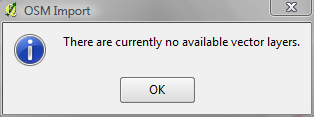
\includegraphics[clip=true, width=8cm]{osm_importdialog}
\end{center}
\end{figure}

In such case there is no vector layer currently loaded. Import must be done
from an opened layer - please open vector layer from which you want to import
data. After layer is opened your second try should give you better result
(don't forget to mark current OSM layer again):

\begin{figure}[ht]
   \begin{center}
   \caption{Import data to OSM dialog \nixcaption}\label{fig:osmimporttoosm}\smallskip
   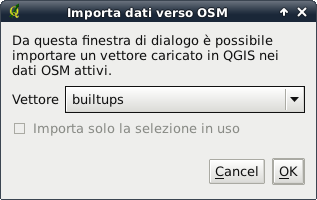
\includegraphics[clip=true, width=8cm]{osm_importtoosmdialog}
\end{center}
\end{figure}

Submit dialog to start the process of OSM data importing.
Reject it if you are not sure you want to import something.


